\subsection{Rosemary}
\label{reuse-rosemary}

\paragraph{Goodness of fit}
To make clear how well Rosemary can be fitted to the \project{} first the functions of the current implementation will be described.
As said in the previous section the system encompasses domain specific data and processing management.
The shear amount of available data and metadata is what makes the data management in this case a challenge.

Data management challenges are tackled by providing extensive search, filter, and selection functionality.
Submissions management is handled by automatically bundling submissions into processings which are then fed to one or multiple applications.
Lastly, notifications and messaging are supported.
Notifications provide users with system status information. 
For example, progress updates during a data import or when receiving a message.
Messaging should enable collaborative work by wrapping research communication inside the same system as where the data resides.

Compared to the functional design (section \ref{function-design}) the most critical part of the system, data management, is mostly covered by Rosemary.
Datasets are bound to \emph{workspaces}, these have an owner and members which can all view the data inside, effectively restricting data access.
To enable the search and filtering a specific model for raw data storage is used and supplemented with an extensive tagging system.
The flexibility of this system means that part of the request and the whole data management requirements can be implemented with minimal changes.

User management can be wholly reused but will need extensions to provide for the necessary user roles.
Furthermore, request and publication management will need to be introduced into the system.

\begin{figure}[!hb]
	\centering
	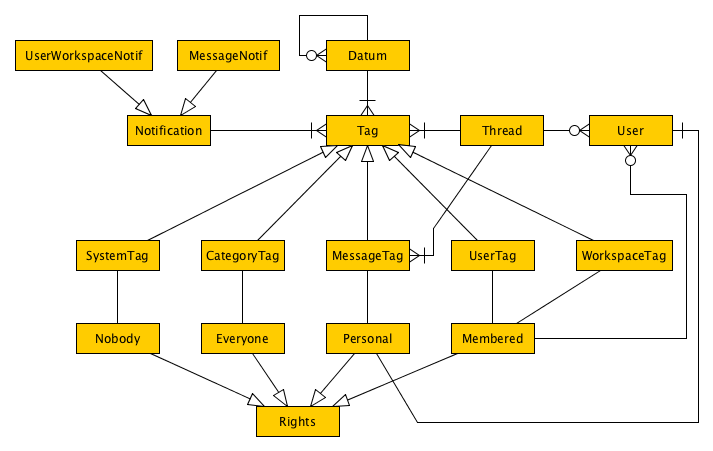
\includegraphics[width=1.0\linewidth]{images/datamodel-clean}
	\caption{
		Rosemary data model with domain specific items removed.
		Describes the workspace, tagging, datum, and notification models.
		The unedited Rosemary data model can be found in appendix \ref{unedited-datamodel}.
	}
	\label{fig:reuse-rosemary-dm}
\end{figure}

\paragraph{Data model}
Figure \ref{fig:reuse-rosemary-dm} depicts the Rosemary data model where the surplus domain specific items are removed.
A full view of the data model can be seen in appendix \ref{unedited-datamodel}.
Implementation is done in mongoDB, a document-oriented database.
The data model and its implementation provide some interesting possibilities.
What is described in figure \ref{fig:reuse-rosemary-dm} as a {\tt Datum} is a single piece of raw data, \ie{} a row in a relational database.
This data can be reused and tracked endlessly by applying a {\tt Tag} object.
For example, access control can be applied by tagging a {\tt Datum} with a {\tt WorkspaceTag} which is owned by a {\tt User}.

Many different constructs of this sort can be achieved without ever touching the structure of the actual model itself.
The reuse in the \ivfsystem{} relies heavily on this concept, which means only slight changed had to be made to the original data objects.